In this section we firstly describe the settings associated to our experimental evaluation and, successively, we report the obtained results and the associated discussion considering the study area introduced in Section~\ref{sec:data} and the competing approaches introduced in Section~\ref{sec:relatedwork}.

\subsection{Experimental settings}
\label{ssec:expe-settings}
With the aim to assess the performances of recent UDA strategies in the context of temporal transfer learning for land cover mapping from SITS data, we have considered the state-of-the-art methods described in Section~\ref{sec:relatedwork}.

About the evaluated methods, we couple the GFK approach with two different classification methods: a Random Forest (RF) and a Multi-layer perceptron (MLP). The latter has two fully connected layers of 512 neurons each (with ReLU activation function) and an output layer (with softmax) to perform the final classification. Both DANN and ADDA are equipped with a backbone especially tailored to manage satellite image time series data. To this end, we adopt the TempCNN model recently proposed in~\cite{Pelletier19}. In addition, we also consider two baseline scenarios in which: i) a supervised classification model is trained with only source data and directly deployed on target data and (only $\mathcal{D}_s$) and ii) a supervised classification model is trained on labelled target data and deployed on the rest of the target examples (only $\mathcal{D}_t$). The former constitutes a straightforward baseline that does not take into account the necessity to deal with data distribution shift while, the latter represents the maximum performances we can (theoretically) achieve if we have label knowledge associated to $\mathcal{D}_t$. For both scenarios we consider as supervised classification methods the TempCNN and RF models.

For neural network approaches, the training stage has been conducted for 300 epochs, with a learning rate of 10$^{-4}$ and a batch size of 64. 
When no domain adaptation is involved, the data is splitted into training, validation and test set considering 50\%, 20\% and 30\% of the original data, respectively. The data was split to avoid possible spatial biases~\cite{IENCO201911}. Weighted F1-score is adopted to evaluate the behaviors of the different competing approaches.

Experiments are carried out on a workstation with a dual Intel (R) Xeon (R) CPU E5-2667v4 with 256 GB of RAM and four TITAN X (Pascal) GPU. All the deep learning methods are implemented using the Python TensorFlow library and run on a single GPU.%, while Random Forest is implemented using Python Scikit-learn library and run only on CPU.

\subsection{Results and discussion}
\label{ssec:results-discussion}
The study was conducted considering two possible configurations: ($\mathcal{D}_s$=2018,$\mathcal{D}_t$=2019) and ($\mathcal{D}_s$=2019,$\mathcal{D}_t$=2018). Nevertheless, only the evaluation for the former configuration is reported and discussed since similar results were obtained considering both configurations.

Table~\ref{tab:uda_methods} reports the results, in terms of weighted F1-score, achieved by the different competing methods. For scenario (only $\mathcal{D}_s$), we can observe that deploying models learnt on  SITS data from 2018 ($\mathcal{D}_s$) to SITS data coming from 2019 ($\mathcal{D}_t$) perform poorly. Generally, we can note more than 15 points of differences between the models trained w.r.t. this scenario and the models trained on $\mathcal{D}_t$ (scenario only $\mathcal{D}_t$). This fact clearly underlines that a serious shift in the data distribution occurs between 2018 and 2019. 

\begin{table}[!htb]
\centering
\small
\begin{tabular}{|c|c|c|c|} \hline
\textbf{Scenario} & \textbf{Method} & \textbf{F1-score} & \textbf{Training Time } \\  \hline
\multirow{2}{*}{Only $\mathcal{D}_s$} & TempCNN & 67.1 & 27 mins.\\ \cline{2-4}
                                      & RF & 67.1 & 2 mins.\\ \hline \hline
\multirow{2}{*}{w/ UDA}  & GFK + MLP & 65.8 & 146 mins.\\ \cline{2-4}
 & GFK + RF & 76.7 & 14 mins.\\ \cline{2-4}
    & ADDA & 80.6 & 650 mins.\\ \cline{2-4}
    & DANN & \textbf{83.7} & 337 mins.\\ \hline \hline
\multirow{2}{*}{Only $\mathcal{D}_t$} & TempCNN & \underline{88.2} & 26 mins.\\ \cline{2-4}
                    & RF & 85.7 & 2 mins.\\ \hline 
\end{tabular}
\caption{Weighted F1-score and training time of the competing approaches. The best F1-score score, for UDA methods, is highlighted in bold; the best score for supervised classification method calibrated on $\mathcal{D}_t$ is underlined. %($\mathcal{D}_s$=2018,$\mathcal{D}_t$=2019). 
\label{tab:uda_methods}}
\end{table}

Regarding transfer learning with the UDA methods (scenario w/ UDA), we can see that the majority of the strategies ameliorate the performances on the target domain. The best results are achieved by the DANN strategy that, exploiting its ability to extract domain invariant features, reduces the gap performances up to less than 5 points w.r.t. the best model (TempCNN) trained directly on the target domain.

\begin{figure}[htb]
  \centering
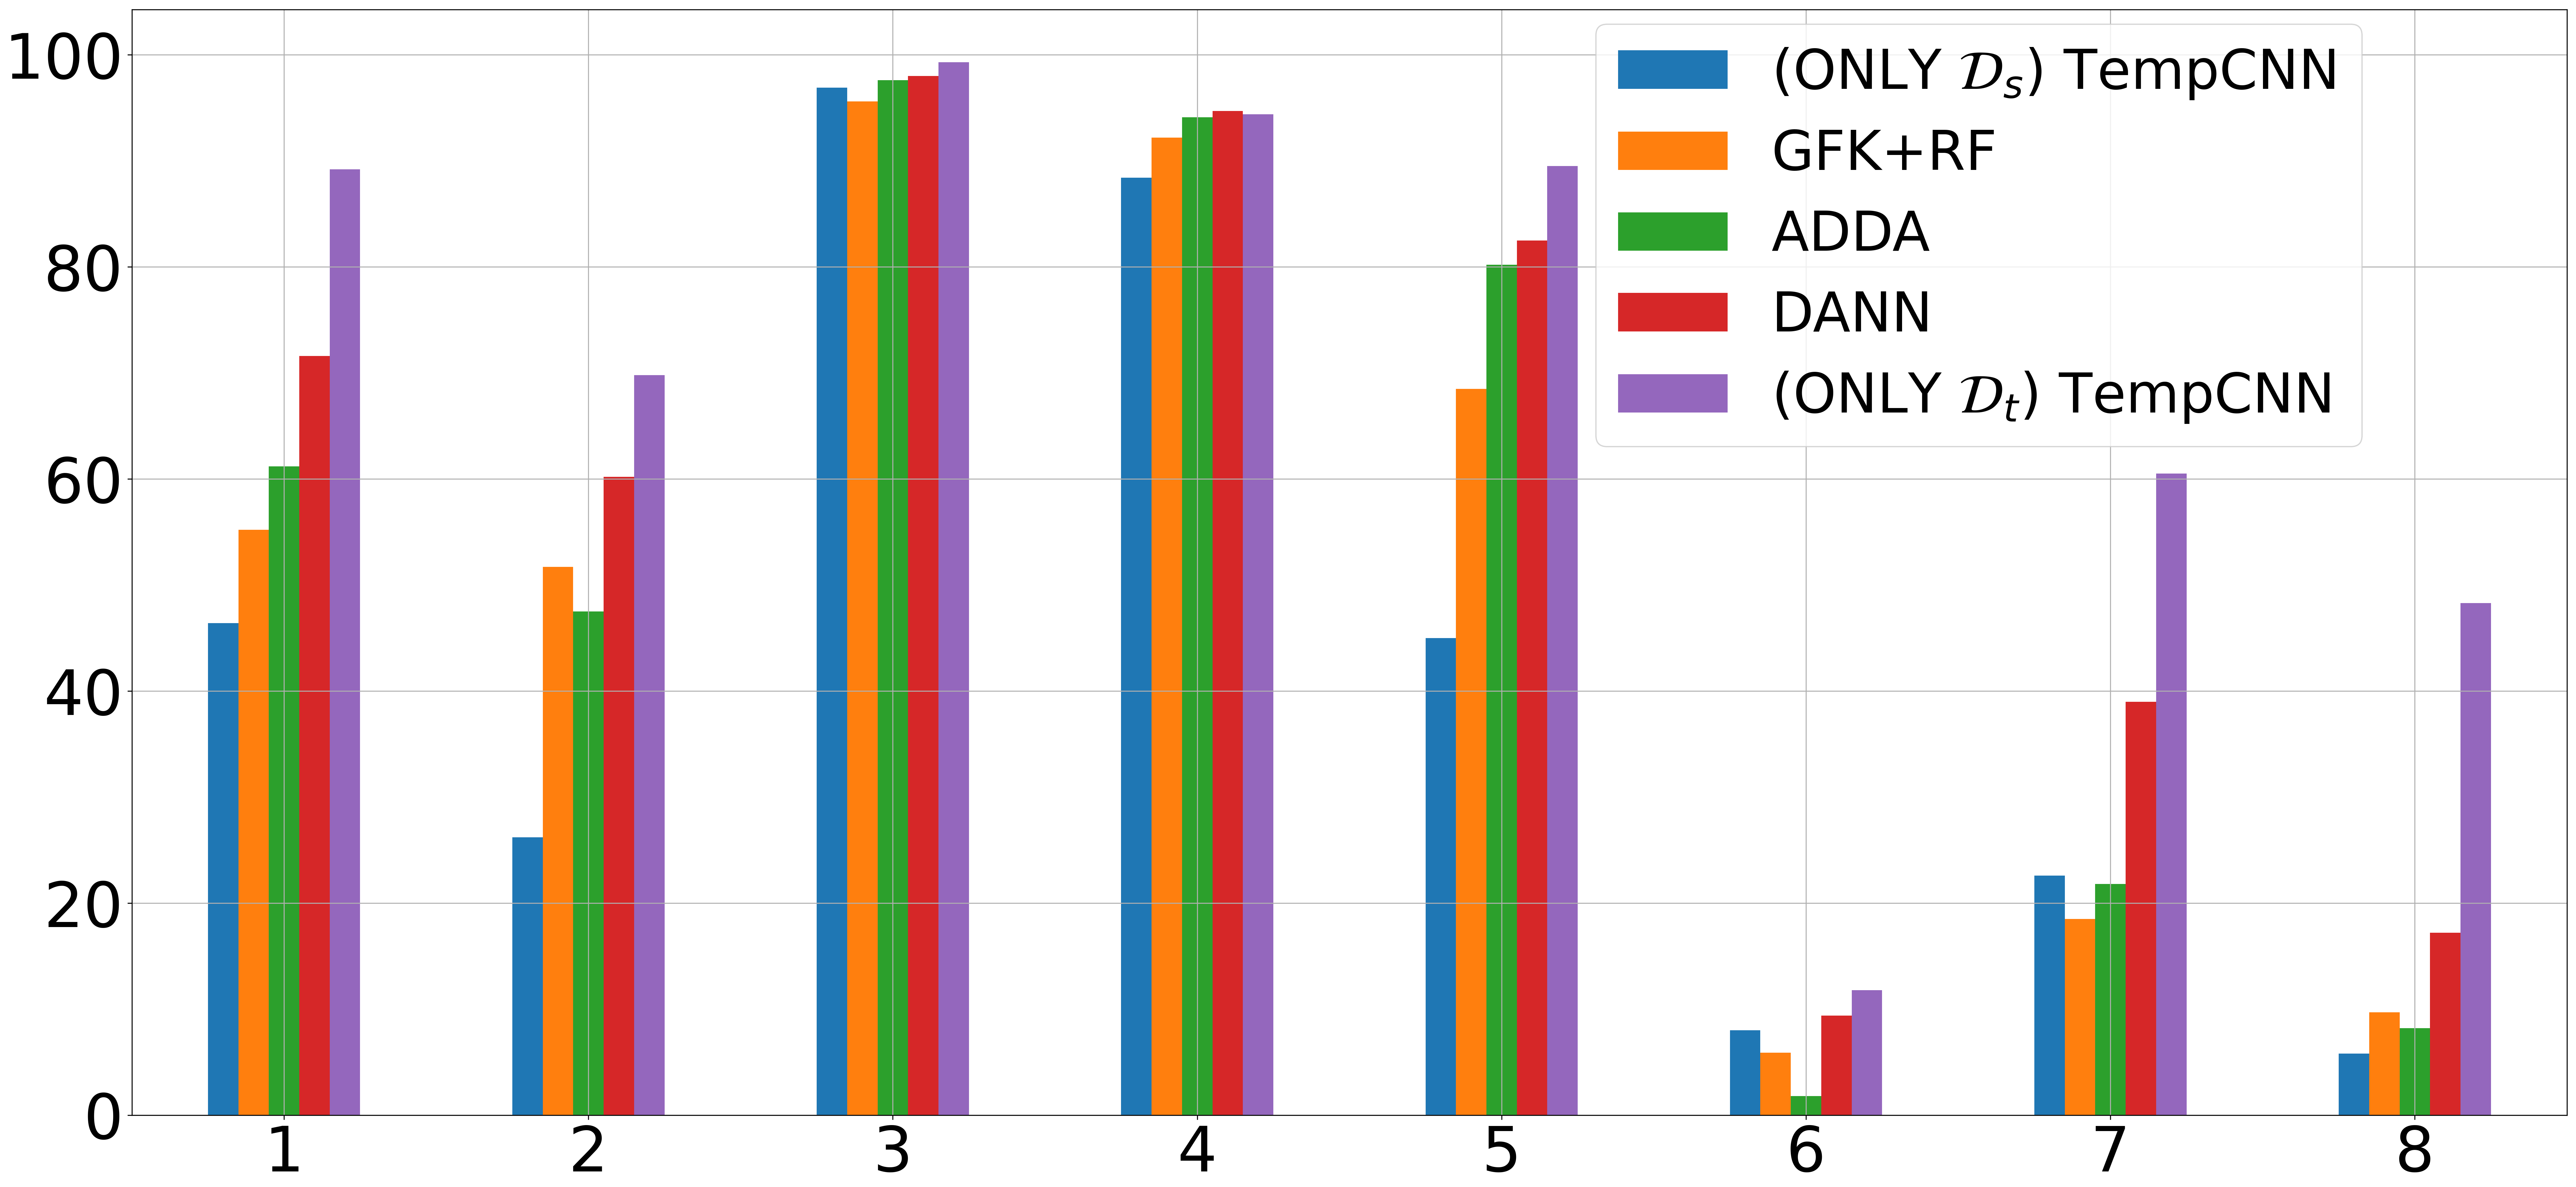
\includegraphics[width=.95\columnwidth]{Figures/analyse_par-classe300_light_rognee.png}
\caption{Per class F1-score, ($\mathcal{D}_s$,$\mathcal{D}_t$) = (2018,2019).}
\label{fig:perClass}
\end{figure}

Figure~\ref{fig:perClass} depicts the per class results, in terms of weighted F1-score and computing time, of the different competing approaches. Firstly, we can note that some classes (\textit{3-Water}, \textit{4-Forest} and \textit{6-Orchard}) seem to exhibit unchanged radiometric distributions between 2018 and 2019 while, the rest of the classes pose some challenges when the model is transferred (i.e. \textit{1-Built}, \textit{7-Crop} and \textit{8-Other Vegegation}). Secondly, we can observe that DANN systematically achieves better performances than all the other competing approaches on the more challenging land cover classes. Finally, we can also advance the hypothesis that the best transfer (at class level) seems to be related to the amount of labelled examples we can access to in the source domain. For instance, UDA methods provide a notable improvement on class \textit{5-Vine} that is the third more represented land cover class in the source domain.

% Please add the following required packages to your document preamble:
% \usepackage{multirow}
% \usepackage[table,xcdraw]{xcolor}
% If you use beamer only pass "xcolor=table" option, i.e. \documentclass[xcolor=table]{beamer}
% \usepackage[normalem]{ulem}
% \useunder{\uline}{\ul}{}




